%!TEX root = ../../thesis.tex

Monte Carlo (MC) event generators provide a fully-exclusive hadron-level simulation of 
\pp collision events at the LHC \cite{MCnet:general}. This section will describe the 
basic features of a simulated event, before discussing some more advanced techniques 
that shall be used throughout the thesis.



\subsection{The anatomy of an event}

\Figure~\ref{fig:mcevent} shows how the MC event generation is factorised into 
several components, each describing a certain regime of momentum transfer.

\begin{figure}[p]
	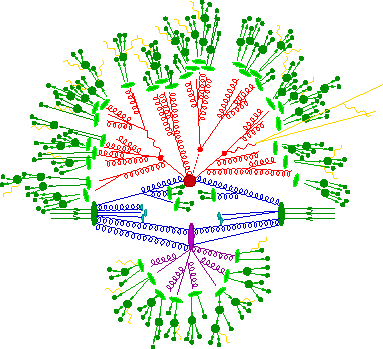
\includegraphics[width=\hugefigwidth]{tex/tools/event}
	\caption{Schematic diagram of a simulated \ttH event, showing how factorisation allows 
	the physics at different scales of momentum transfer $Q$ to be treated independently 
	\cite{MCnet:MatchingLectures}.
	At high-$Q$ is the hard scatter (red circle). As the scale evolves down, partons are 
	radiated in the initial state (blue) and final state (red). At low-$Q$, incoming 
	partons are confined to the beam protons, while outgoing partons hadronise (green 
	blobs). The underlying event comprises multiple partonic interactions (purple blob) 
	and beam remnants (blue blobs). Photons and leptons (yellow) are also radiated.}
	\label{fig:mcevent}
\end{figure}

\begin{description}
\item[Hard scatter] \hfill \\
	The high scale process can be selected as desired (\eg Higgs boson production via 
	gluon-gluon fusion). The relevant parton-level matrix elements (MEs) are calculated 
	using fixed order perturbative QCD, either by the event generator itself or an 
	external program. Historically, these MEs were usually LO, though improvements are 
	discussed in Sections~\ref{sec:mc:merging} and \ref{sec:mc:matching}.
\item[Parton distribution functions (PDFs)] \hfill \\
	Incoming parton momenta are sampled from a proton PDF, usually probed at the 
	scale of the hard scatter ($\muf = Q$). The LHAPDF interface \cite{LHAPDF} provides 
	access to the PDFs of several fitting collaborations, such as CTEQ \cite{CTEQ}, 
	MSTW \cite{MSTW} and NNPDF \cite{NNPDF}. PDFs differ because they are fit with 
	different subsets of experimental data, massive quark treatments, parametrisation 
	models and $\alphaS \parenths{\mZ}$ values.
\item[Final state radiation (FSR)] \hfill \\
	Soft and collinear radiation from outgoing partons is simulated by a universal parton 
	shower, evolving the scale from the hard scatter to the hadronisation scale of 
	\about\unit{1}{\GeV}. The successive emissions are ordered to avoid double-counting --
	typical order parameters are virtuality, transverse momentum and opening angle.

	For the correct treatment of soft emissions, it is vital to preserve colour 
	coherence. This is inherent in an angular ordered shower, but must be manually 
	implemented otherwise. Alternatively, a \textit{dipole shower} considers emissions 
	from colour-connected pairs of partons, and is also inherently coherent.
\item[Initial state radiation (ISR)] \hfill \\
	Soft and collinear radiation from incoming partons is similarly described by a parton 
	shower. However, the small probability of evolving two partons with the kinematics 
	required by the hard process necessitates a \textit{backwards evolution}. Thus, the 
	probability that a parton originated from one of higher momentum and lower scale is 
	calculated, rather than an emission probability.
\item[Hadronisation] \hfill \\
	The confinement of partons to hadrons is non-perturbative, and must be described by a 
	hadronisation model. The \textit{string model} stretches strings between colour 
	partners. At some distance it becomes favourable to convert the potential energy to a 
	\HepProcess{\Pquark \APquark} pair, breaking the string. Once there is insufficient 
	energy to create \HepProcess{\Pquark \APquark} pairs, the hadrons `freeze out'. The 
	\textit{cluster model} splits gluons into \HepProcess{\Pquark \APquark} pairs, which 
	group into colourless clusters with a mass spectrum predicted by QCD. These 
	clusters then decay to the physical hadrons. Note that all hadronisation models 
	require tuning to experimental data.
\item[Hadron and \Ptau decays] \hfill \\
	Many of the hadrons produced during hadronisation are unstable, and must be decayed to
	particles that are stable on a detector traversal timescale, while observing 
	conservation laws and measured branching ratios. Similarly, the \Ptau lepton must be 
	decayed, hadronically or leptonically.
\item[Multiple partonic interactions (MPI)] \hfill \\
	The \textit{underlying event} (UE) is the additional soft hadronic activity caused by 
	partons inactive in the hard scatter. It comprises the breakup of the beam remnants 
	and \textit{multiple partonic interactions} (MPI) between the protons. The size of 
	the MPI activity is correlated to the scale of the hard scatter. 

	In order to calculate the number of additional interactions, the spatial distribution 
	of partons within the proton must be modelled, the impact parameter of the \pp 
	collision must be known, and an IR cut-off must be imposed. This requires 
	non-perturbative models that must be tuned to experimental data.
\item[QED radiation] \hfill \\
	Electrically charged particles can emit photons at any stage of the event generation.
\end{description}



\subsection{Summary of event generators}
\label{sec:mc:generators}

Three event generators are commonly used at the LHC, mainly differing in their 
choice of hadronisation and MPI models, and their parton shower order parameter. 
Efforts to rewrite the older Fortran-based programs in \cpp have led to a generation of 
`out-of-date' Fortran programs that are no longer actively developed. Even so, they are 
still in common usage, and so are included in the descriptions below.

\begin{description}
\item[Herwig] \hfill \\
	\fherwig (Fortran) \cite{fHerwig} and \herwigpp (\cpp) \cite{Herwig++} both employ an 
	angular ordered parton shower and a cluster hadronisation model. An MPI model is 
	included in \herwigpp, but in \fherwig this was provided by \jimmy \cite{Jimmy}.
\item[Pythia] \hfill \\
	\pythia{6} (Fortran) \cite{Pythia6} and \pythia{8} (\cpp) \cite{Pythia8} both use a 
	string hadronisation model and an advanced MPI model. \pythia{8} uses a dipole 
	shower ordered in transverse momentum, whereas \pythia{6} offers a choice of 
	virtuality or transverse momentum ordered parton showers with colour coherence 
	implemented manually.
\item[Sherpa] \hfill \\
	\sherpa (\cpp) \cite{Sherpa} uses a dipole shower ordered in transverse momentum, 
	which is convenient for multi-leg merging (see \Section~\ref{sec:mc:merging}). It 
	uses a cluster hadronisation model and an MPI model similar to that of \pythia{8}.
\end{description}



\subsection{Multi-leg merging}
\label{sec:mc:merging}

Although a parton shower excellently describes the emissions of large numbers of soft and 
collinear partons, it fails to accurately model hard and isolated emissions. It can be 
desirable to describe these using fixed order MEs, which are better suited to the 
task. In doing so, a couple of immediate issues arise. First, we require a smooth 
transition from the emissions of an ME to those of the parton shower. Second, each 
ME is inclusive, and attempting to combine MEs of differing multiplicity 
naturally leads to problems of double counting.

By using a merging prescription, such as the CKKW-L algorithm \cite{CKKW,Lonnblad:2002} 
employed by \sherpa or the MLM algorithm \cite{Merging} employed by \alpgen \cite{Alpgen} 
and \madgraph \cite{MadGraph}, it is possible to consistently combine LO matrix 
elements with differing multiplicities, whilst matching to the parton shower correctly. 
This does require the introduction of a merging scale though. This scale separates the 
ME and parton shower descriptions of the emissions, though the details of the 
separation depend upon the merging prescription.



\subsection{NLO matching}
\label{sec:mc:matching}

It is also possible to match an NLO ME to a parton shower, to improve the accuracy
of both the normalisation and distribution of observables \cite{Nason:2012}. Such a 
calculation must include the LO, virtual-loop and real-emission diagrams, while 
mapping smoothly onto the parton shower for soft emissions. There are currently two valid 
matching prescriptions:

\begin{description}
\item[MC@NLO] \hfill \\
	Simply adding a parton shower to an NLO ME introduces double counting of 
	emissions. The \mcatnlo method compensates for this overlap through a correction to 
	the NLO calculation. This renders the ME dependent upon the parton shower 
	used in the MC event generator. It also introduces negatively weighted events.

	Originally implemented in the \mcatnlo program for matching to \fherwig 
	\cite{MCatNLO-Herwig} and \herwigpp \cite{MCatNLO-Herwig++}, the method has now been 
	automated within the \amcatnlo program \cite{aMCatNLO} and extended for use with 
	\pythia{6} and \pythia{8} \cite{MCatNLO-Pythia}. It is now also included in \sherpa.
\item[POWHEG] \hfill \\
	The \powhegmethod method requires the hardest emission to always be generated by 
	the ME. It achieves the correct hard and soft behaviour by convolving the LO
	ME with a modified Sudakov factor, and then reweighting the differential cross 
	section to the NLO result. Thus the ME is independent of the subsequent 
	parton shower. However, if the parton shower is not transverse momentum ordered, it is
	necessary to use truncated and vetoed parton showers to correctly fill the phase 
	space.

	Originally implemented in \powhegbox \cite{Powheg-method,Powheg-method2,PowhegBox}, 
	variants are now also included in \herwigpp and \sherpa.
\end{description}



\subsection{Additional considerations}
\label{sec:mc:other}

\begin{description}
\item[Detector simulation] \hfill \\
	In order to compare MC events to experimental events recorded at the LHC, 
	it is vital to simulate how the outgoing particles interact with the detector. This 
	is also necessary to calibrate the detector response and estimate efficiencies. 
	\geant \cite{GEANT4,ATLAS-simulation} is used to simulate the energy deposition of 
	each particle during its trajectory through the ATLAS detector (see 
	\Chapter~\ref{chap:experiment}). Since long-lived particles will decay \textit{en 
	route}, particles with lifetime \unit{$c\tau > 10$}{\milli\metre} are decayed by 
	\geant rather than the MC generator. The majority of the simulation time is 
	spent modelling the complex calorimeter geometry; in some cases the simulation is 
	performed by \atlfast \cite{Atlfast}, which contains a simplified calorimeter 
	simulation.

	\textit{Digitisation} converts the energy deposition into readout voltages and 
	currents. Following this, the events can be treated like experimental collision 
	events.
\item[Pile-up simulation] \hfill \\
	As described in \Chapter~\ref{chap:experiment}, each LHC bunch crossing can 
	result in soft proton-proton interactions, known as \textit{pile-up}, in addition to 
	the hard process. This obscures the interesting physics and is important to model 
	accurately.

	In-time pile-up (same bunch crossing as the hard process) is modelled by overlaying 
	simulated energy deposits from soft \pp interactions generated with \pythia{8}. The 
	number of overlaid events depends upon the beam conditions (see 
	\Section~\ref{sec:dataset}).

	Out-of-time pile-up (different bunch crossing to the hard process) affects detector 
	sub-systems whose latency is longer than the bunch spacing. For such sub-systems, 
	signals from out-of-time pile-up are overlaid with corresponding time shifts; again 
	this depends on the beam conditions.
\end{description}



\subsection{Parton shower tuning study}
\label{sec:mc:ps_tuning}

When studying MC modelling uncertainties in the ggF process (see \Section~\ref{sec:ggf_mc}), 
a discrepancy was observed at high jet multiplicity between \meps{\powhegbox}{\pythia{8}} 
and \meps{\powhegbox}{\pythia{6}} (see the green and black lines in 
\Figure~\ref{fig:mc:ps_tuning}). It is also observed in other electroweak processes.

\begin{figure}[t]
	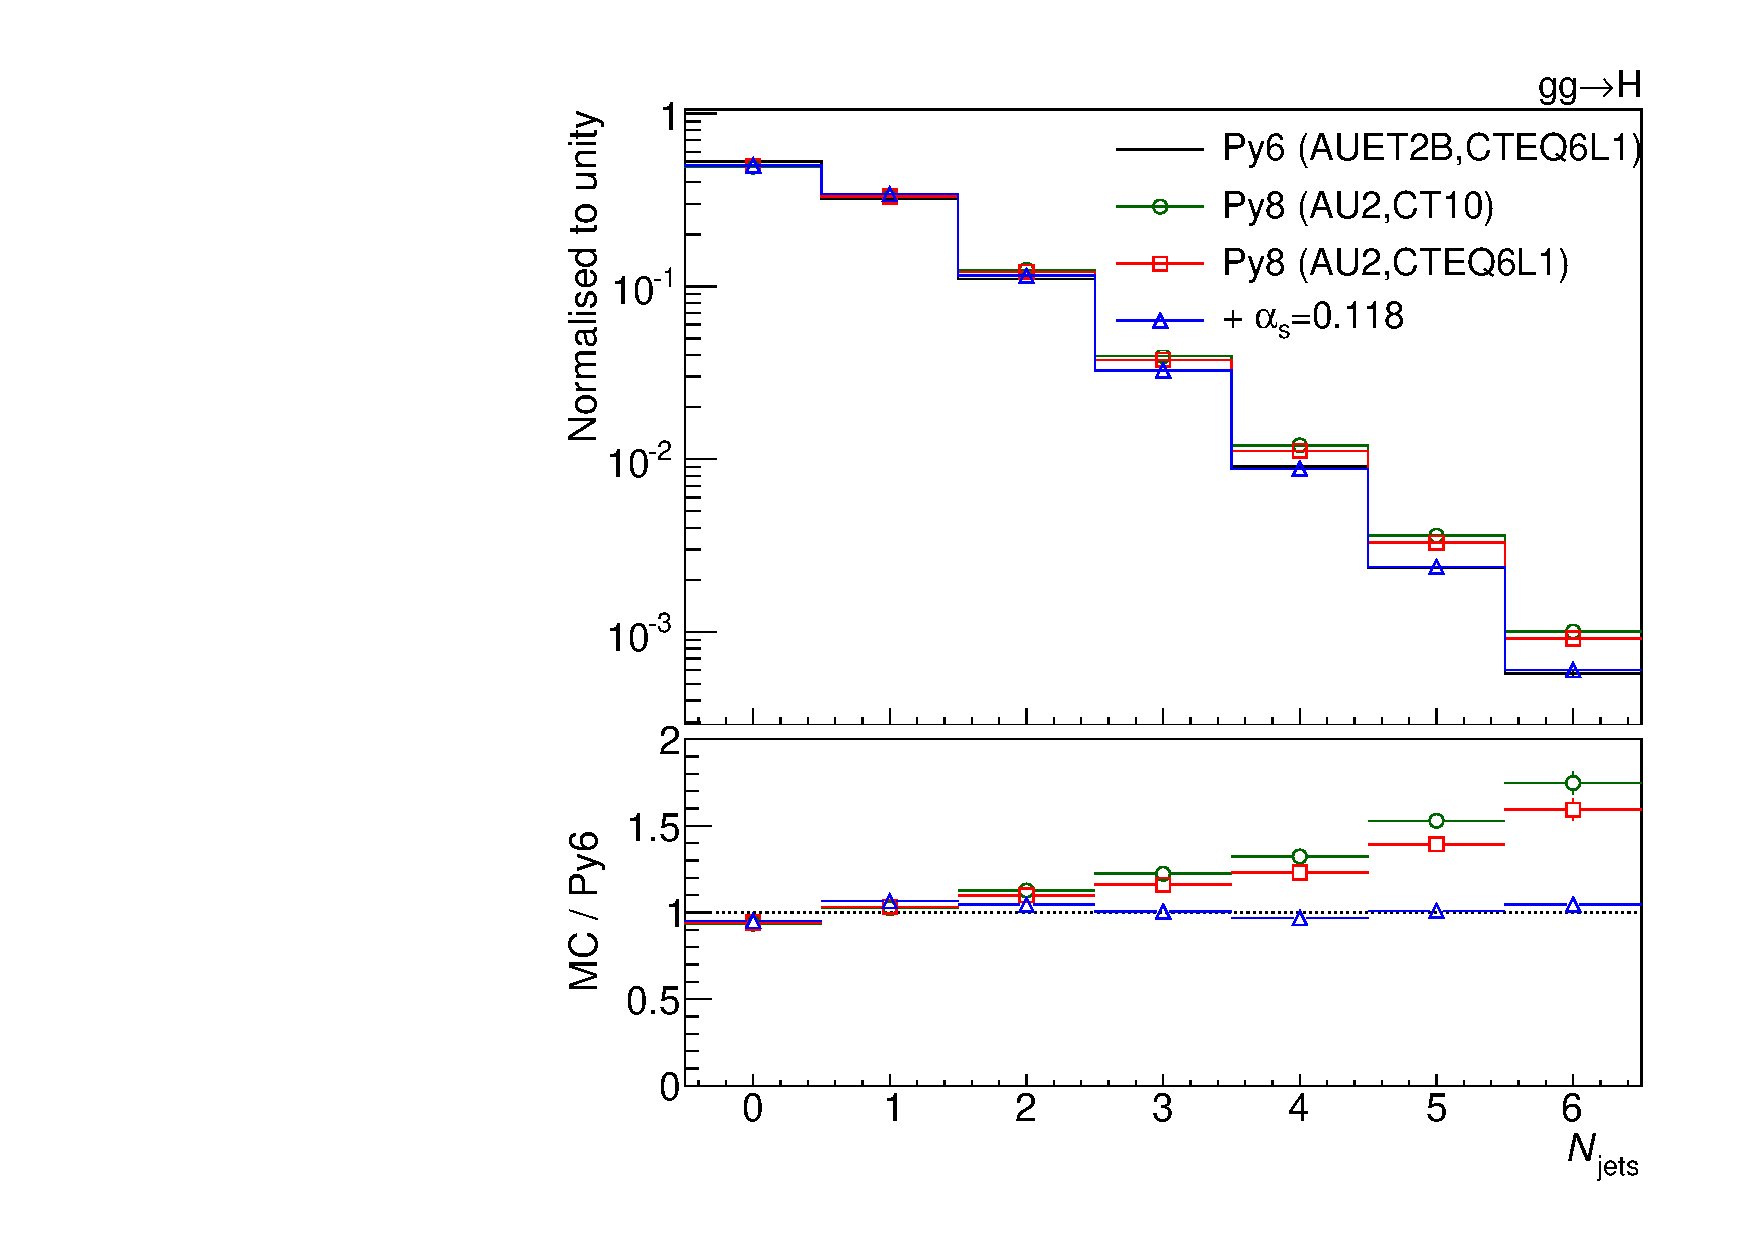
\includegraphics[width=\smallfigwidth]{tex/signal/matching}
	\caption{Jet multiplicity produced by \meps{\powhegbox}{\pythia{8}} with a selection 
	of shower tunes. The green circles correspond to the tune used in the analysis. The red 
	squares change the parton shower PDFs from CT10 to CTEQ6L1. The blue triangles 
	additionally change the parton shower $\alphaS\parenths{\mZ}$ from 0.137 to 0.118 (in 
	agreement with \powhegbox). \meps{\powhegbox}{\pythia{6}} is shown in black for 
	reference, and is in good agreement with \meps{\powhegbox}{\fherwig}.}
	\label{fig:mc:ps_tuning}
\end{figure}

The hadronisation and UE models of standalone \pythia{8} have been tuned to ATLAS 
UE data with a variety of PDF sets (known as AU2 tunes) \cite{ATLAS:tune:2012}.
However, the parton shower was not tuned since the default settings successfully described 
experimental data. 

When modelling ggF with \powhegbox, the AU2-CT10 tune was used in order to match the 
PDFs used in the matrix element calculation. Technically speaking, a dedicated 
\meps{\powhegbox}{\pythia{8}} tune should have been used, but this was unavailable. 
Unfortunately, a couple of issues had a negative impact on the NLO-PS matching. First, 
the parton shower evolves \alphaS at LO, whilst NLO PDFs were used in the shower. 
Second, there was a mismatch between the \alphaS used in \powhegbox, 
$\alphaS\parenths{\mZ} = 0.118$, and the default value in the parton shower, 
$\alphaS\parenths{\mZ} = 0.137$. The effect of these issues is shown in 
\Figure~\ref{fig:mc:ps_tuning}.

Identification of this poor matching has led to improvements in the latest round of MC 
tuning, where dedicated \meps{\powhegbox}{\pythia{8}} tunes are fit using an adjusted 
parton shower \cite{ATLAS:tune:2013}.


